
%% bare_conf.tex
%% V1.4b
%% 2015/08/26
%% by Michael Shell
%% See:
%% http://www.michaelshell.org/
%% for current contact information.
%%
%% This is a skeleton file demonstrating the use of IEEEtran.cls
%% (requires IEEEtran.cls version 1.8b or later) with an IEEE
%% conference paper.
%%
%% Support sites:
%% http://www.michaelshell.org/tex/ieeetran/
%% http://www.ctan.org/pkg/ieeetran
%% and
%% http://www.ieee.org/

%%*************************************************************************
%% Legal Notice:
%% This code is offered as-is without any warranty either expressed or
%% implied; without even the implied warranty of MERCHANTABILITY or
%% FITNESS FOR A PARTICULAR PURPOSE! 
%% User assumes all risk.
%% In no event shall the IEEE or any contributor to this code be liable for
%% any damages or losses, including, but not limited to, incidental,
%% consequential, or any other damages, resulting from the use or misuse
%% of any information contained here.
%%
%% All comments are the opinions of their respective authors and are not
%% necessarily endorsed by the IEEE.
%%
%% This work is distributed under the LaTeX Project Public License (LPPL)
%% ( http://www.latex-project.org/ ) version 1.3, and may be freely used,
%% distributed and modified. A copy of the LPPL, version 1.3, is included
%% in the base LaTeX documentation of all distributions of LaTeX released
%% 2003/12/01 or later.
%% Retain all contribution notices and credits.
%% ** Modified files should be clearly indicated as such, including  **
%% ** renaming them and changing author support contact information. **
%%*************************************************************************

% *** Authors should verify (and, if needed, correct) their LaTeX system  ***
% *** with the testflow diagnostic prior to trusting their LaTeX platform ***
% *** with production work. The IEEE's font choices and paper sizes can   ***
% *** trigger bugs that do not appear when using other class files.       ***                          ***
% The testflow support page is at:
% http://www.michaelshell.org/tex/testflow/

\documentclass[conference]{IEEEtran}
% Some Computer Society conferences also require the compsoc mode option,
% but others use the standard conference format.
%
% If IEEEtran.cls has not been installed into the LaTeX system files,
% manually specify the path to it like:
% \documentclass[conference]{../sty/IEEEtran}

% Some very useful LaTeX packages include:
% (uncomment the ones you want to load)

% *** MISC UTILITY PACKAGES ***
%
%\usepackage{ifpdf}
% Heiko Oberdiek's ifpdf.sty is very useful if you need conditional
% compilation based on whether the output is pdf or dvi.
% usage:
% \ifpdf
%   % pdf code
% \else
%   % dvi code
% \fi
% The latest version of ifpdf.sty can be obtained from:
% http://www.ctan.org/pkg/ifpdf
% Also, note that IEEEtran.cls V1.7 and later provides a builtin
% \ifCLASSINFOpdf conditional that works the same way.
% When switching from latex to pdflatex and vice-versa, the compiler may
% have to be run twice to clear warning/error messages.

% *** CITATION PACKAGES ***
%
\usepackage{cite}

% *** GRAPHICS RELATED PACKAGES ***
%
\ifCLASSINFOpdf
 \usepackage[pdftex]{graphicx}
  % declare the path(s) where your graphic files are
  % \graphicspath{{../pdf/}{../jpeg/}}
  % and their extensions so you won't have to specify these with
  % every instance of \includegraphics
  % \DeclareGraphicsExtensions{.pdf,.jpeg,.png}
\else
  % or other class option (dvipsone, dvipdf, if not using dvips). graphicx
  % will default to the driver specified in the system graphics.cfg if no
  % driver is specified.
  % \usepackage[dvips]{graphicx}
  % declare the path(s) where your graphic files are
  % \graphicspath{{../eps/}}
  % and their extensions so you won't have to specify these with
  % every instance of \includegraphics
  % \DeclareGraphicsExtensions{.eps}
\fi
% graphicx was written by David Carlisle and Sebastian Rahtz. It is
% required if you want graphics, photos, etc. graphicx.sty is already
% installed on most LaTeX systems. The latest version and documentation
% can be obtained at: 
% http://www.ctan.org/pkg/graphicx
% Another good source of documentation is "Using Imported Graphics in
% LaTeX2e" by Keith Reckdahl which can be found at:
% http://www.ctan.org/pkg/epslatex
%
% latex, and pdflatex in dvi mode, support graphics in encapsulated
% postscript (.eps) format. pdflatex in pdf mode supports graphics
% in .pdf, .jpeg, .png and .mps (metapost) formats. Users should ensure
% that all non-photo figures use a vector format (.eps, .pdf, .mps) and
% not a bitmapped formats (.jpeg, .png). The IEEE frowns on bitmapped formats
% which can result in "jaggedy"/blurry rendering of lines and letters as
% well as large increases in file sizes.
%
% You can find documentation about the pdfTeX application at:
% http://www.tug.org/applications/pdftex

% *** MATH PACKAGES ***
%
%\usepackage{amsmath}

% *** SPECIALIZED LIST PACKAGES ***
%
%\usepackage{algorithmic}

% *** ALIGNMENT PACKAGES ***
%
%\usepackage{array}


% IEEEtran contains the IEEEeqnarray family of commands that can be used to
% generate multiline equations as well as matrices, tables, etc., of high
% quality.

% *** SUBFIGURE PACKAGES ***
%\ifCLASSOPTIONcompsoc
%  \usepackage[caption=false,font=normalsize,labelfont=sf,textfont=sf]{subfig}
%\else
%  \usepackage[caption=false,font=footnotesize]{subfig}
%\fi
% subfig.sty, written by Steven Douglas Cochran, is the modern replacement
% for subfigure.sty, the latter of which is no longer maintained and is
% incompatible with some LaTeX packages including fixltx2e. However,
% subfig.sty requires and automatically loads Axel Sommerfeldt's caption.sty
% which will override IEEEtran.cls' handling of captions and this will result
% in non-IEEE style figure/table captions. To prevent this problem, be sure
% and invoke subfig.sty's "caption=false" package option (available since
% subfig.sty version 1.3, 2005/06/28) as this is will preserve IEEEtran.cls
% handling of captions.
% Note that the Computer Society format requires a larger sans serif font
% than the serif footnote size font used in traditional IEEE formatting
% and thus the need to invoke different subfig.sty package options depending
% on whether compsoc mode has been enabled.
%
% The latest version and documentation of subfig.sty can be obtained at:
% http://www.ctan.org/pkg/subfig




% *** FLOAT PACKAGES ***
%
%\usepackage{fixltx2e}
% fixltx2e, the successor to the earlier fix2col.sty, was written by
% Frank Mittelbach and David Carlisle. This package corrects a few problems
% in the LaTeX2e kernel, the most notable of which is that in current
% LaTeX2e releases, the ordering of single and double column floats is not
% guaranteed to be preserved. Thus, an unpatched LaTeX2e can allow a
% single column figure to be placed prior to an earlier double column
% figure.
% Be aware that LaTeX2e kernels dated 2015 and later have fixltx2e.sty's
% corrections already built into the system in which case a warning will
% be issued if an attempt is made to load fixltx2e.sty as it is no longer
% needed.
% The latest version and documentation can be found at:
% http://www.ctan.org/pkg/fixltx2e


%\usepackage{stfloats}
% stfloats.sty was written by Sigitas Tolusis. This package gives LaTeX2e
% the ability to do double column floats at the bottom of the page as well
% as the top. (e.g., "\begin{figure*}[!b]" is not normally possible in
% LaTeX2e). It also provides a command:
%\fnbelowfloat
% to enable the placement of footnotes below bottom floats (the standard
% LaTeX2e kernel puts them above bottom floats). This is an invasive package
% which rewrites many portions of the LaTeX2e float routines. It may not work
% with other packages that modify the LaTeX2e float routines. The latest
% version and documentation can be obtained at:
% http://www.ctan.org/pkg/stfloats
% Do not use the stfloats baselinefloat ability as the IEEE does not allow
% \baselineskip to stretch. Authors submitting work to the IEEE should note
% that the IEEE rarely uses double column equations and that authors should try
% to avoid such use. Do not be tempted to use the cuted.sty or midfloat.sty
% packages (also by Sigitas Tolusis) as the IEEE does not format its papers in
% such ways.
% Do not attempt to use stfloats with fixltx2e as they are incompatible.
% Instead, use Morten Hogholm'a dblfloatfix which combines the features
% of both fixltx2e and stfloats:
%
% \usepackage{dblfloatfix}
% The latest version can be found at:
% http://www.ctan.org/pkg/dblfloatfix




% *** PDF, URL AND HYPERLINK PACKAGES ***
%
%\usepackage{url}
% url.sty was written by Donald Arseneau. It provides better support for
% handling and breaking URLs. url.sty is already installed on most LaTeX
% systems. The latest version and documentation can be obtained at:
% http://www.ctan.org/pkg/url
% Basically, \url{my_url_here}.




% *** Do not adjust lengths that control margins, column widths, etc. ***
% *** Do not use packages that alter fonts (such as pslatex).         ***
% There should be no need to do such things with IEEEtran.cls V1.6 and later.
% (Unless specifically asked to do so by the journal or conference you plan
% to submit to, of course. )


% correct bad hyphenation here
\hyphenation{op-tical net-works semi-conduc-tor}


\begin{document}
%
% paper title
% Titles are generally capitalized except for words such as a, an, and, as,
% at, but, by, for, in, nor, of, on, or, the, to and up, which are usually
% not capitalized unless they are the first or last word of the title.
% Linebreaks \\ can be used within to get better formatting as desired.
% Do not put math or special symbols in the title.
\title{Deep Reinforcement Learning for Browser Tasks}


% author names and affiliations
% use a multiple column layout for up to three different
% affiliations
\author{\IEEEauthorblockN{Minttu Alakuijala}
\IEEEauthorblockA{minttu.alakuijala.14@ucl.ac.uk}\\
\IEEEauthorblockN{Jamie Law}
\IEEEauthorblockA{jamie.law.14@ucl.ac.uk}
\and
\IEEEauthorblockN{Vika Christy}
\IEEEauthorblockA{anastasia.christy.14@ucl.ac.uk}\\
\IEEEauthorblockN{Yuhang Xu}
\IEEEauthorblockA{yuhang.xu.14@ucl.ac.uk}\\
\IEEEauthorblockA{University College London, Computer Science}
\and
\IEEEauthorblockN{Rajind Karunaratne}
\IEEEauthorblockA{rajind.karunaratne.14@ucl.ac.uk}\\
\IEEEauthorblockN{Jun Wang}
\IEEEauthorblockA{j.wang@cs.ucl.ac.uk}
}




% use for special paper notices
%\IEEEspecialpapernotice{(Invited Paper)}




% make the title area
\maketitle

% As a general rule, do not put math, special symbols or citations
% in the abstract
\begin{abstract}
Deep learning is an emerging field that has shown many breakthroughs recently due to the technology available. Within reinforcement learning, deep learning has shown to be effective in game-like environments. The purpose of this study is to investigate the effectiveness of using deep reinforcement learning to train agents on a novel benchmark, Mini World of Bits (developed by OpenAI). This benchmark can be seen as an initial foundation for website interaction which, if mastered, would strongly infer development towards performing automation on tasks in real-world websites and furthering progress towards AI general intelligence. We look at adapting and evaluating deep Q-networks and policy gradient algorithms for this benchmark and then determining each model's success based off an average of the reward function from the environments, ideally looking towards a positive trend through the training process. [potential conclusion based on results]
\end{abstract}

% no keywords
% For peer review papers, you can put extra information on the cover
% page as needed:
% \ifCLASSOPTIONpeerreview
% \begin{center} \bfseries EDICS Category: 3-BBND \end{center}
% \fi
%
% For peerreview papers, this IEEEtran command inserts a page break and
% creates the second title. It will be ignored for other modes.
\IEEEpeerreviewmaketitle

\section{Introduction}
Over the past few years, there has been a monumental shift in technology and how it's being applied to everyday life, of which deep reinforcement learning is a field which has recently shown potential due to the technology available. With typical algorithms, computers are told how to deal with problems, but with deep learning computers are told to teach themselves to deal with these problems. Significant progress has already been demonstrated in experiments on the Universe platform, where agents have been trained via deep reinforcement learning to successfully play Atari games \cite{mnih2013playing}. We have looked to extend the implementation of deep reinforcement learning methods onto browser-based tasks. This introduction will give the reader an insight into the concerned technologies as well as deriving a justified hypothesis. 

\subsection{OpenAI Universe}
Universe is a software platform developed by OpenAI built for training and measuring AI across a wide range of games, websites and other environments. Any program can be turned into a Gym (a toolkit for developing and comparing reinforcement learning algorithms) environment via this platform. It provides the agent's access to programs via a VNC client on a remote desktop (inside a Docker container), allowing the agent to perceive and act on the program the same way a human does by interpreting the pixel values of a screen and producing a combination of keyboard and/or mouse actions. 

The ultimate goal of Universe is to develop a single agent that can apply all of its previous experiences to quickly adapt and master to other unfamiliar environments, which would demonstrate monumental progress towards general intelligence. This differs to other systems which typically fall into the category of "Narrow AI", which are systems that perform well in a specific domain but struggle to adapt to other environments. 

A large number of environments have already been integrated into Universe, such as Atari games, Flash games and Browser based tasks, of which a prominent benchmark is Mini World of Bits.

\subsection{Mini World of Bits}

\begin{figure*}[t]
	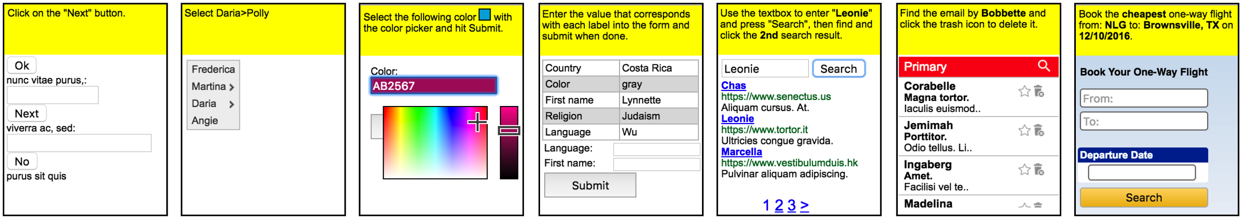
\includegraphics[width=\textwidth, height=\textheight, keepaspectratio]{mwob.png}
	\caption{Example environments from the Mini World of Bits benchmark \cite{mwob}, task prompts are indicated in the yellow section while the white section is the canvas area}
	\label{fig:mwob}
\end{figure*}

Mini World of Bits (MWoB) \cite{mwob} is a new benchmark which consists of a wide range of browser-based tasks, such as clicking a button, entering text, all the way up to more complex tasks such as searching for a flight between dates. It can be seen as an initial foundation that encapsulates the core functionalities of website interactions which, if mastered, would provide strong inference of development towards performing well on real-world websites. The benchmark can be seen as an equivalence to the MNIST dataset \cite{lecun1998gradient} in terms of visual recognition, where the ultimate goal for the agents is to be able to perceive and interpret the provided data in a small, self-contained area to complete the task.

The environments are written in a combination of HTML, JavaScript and CSS, although the agents can not perceive this information via Universe. Each environment is a 210px by 160px webpage, where the yellow section indicates the task prompt and the white section is the canvas area for performing the task (examples of environments can be seen in figure \ref{fig:mwob}). The agents receive visual information which are the raw pixel values of the webpage and then attempt to produce a combination of keyboard or mouse actions to attempt to complete the task. They also receive a reward value based on the task progress, ranging 0 to 1 if the task is completed (dependent on the time taken for completion) and -1 if the task is failed or time has run out.

We have looked into the MWoB benchmark due to its novelty; no results have been published yet for this, in contrast to other Universe environments such as Atari games or Flash games where significant progress has already been demonstrated using deep reinforcement learning \cite{mnih2013playing}.

\subsection{Hypothesis}
Due to the success of deep reinforcement learning in other experiments, we are looking to investigate the effectiveness of using the respective algorithms on the Mini World of Bits benchmark:
\begin{center}
\textit{"Deep Reinforcement Learning would be effective in the Mini World of Bits benchmark"}
\end{center}

\section{Related work}
Subsection text here.

\section{Methodology}

\subsection{Environments}

\subsection{Action spaces}

\subsection{Implemented models}

\subsection{Input processing}

\subsection{Reward manipulation}

\subsection{Supervised methods}

\subsection{Metrics}

\subsection{Benchmarks}

\section{Results}

\section{Analysis}

\subsection{Limitations}

\section{Conclusion and future work}
\subsection{Conclusion}
Following from the analysis of our results, we can conclude that...
\subsection{Future work}
The novelty of the benchmark indicates still a wide area of progress that can be made, as such there are many future possibilities to expand upon the current state of our project:
\subsubsection{Continuous action spaces}
As we have only discussed discrete action spaces, we would invest more research into implementing continuous action spaces. We are still currently looking into the full implementation and training of an agent via a \textbf{Deep Deterministic Policy Gradient} algorithm \cite{lillicrap2015continuous}, which is specifically designed for continuous action spaces and has shown to be very effective in other non-MWoB environments that use continuous actions, such as the inverted pendulum experiment \cite{pendulum} where the objective is to provide a magnitude to balance the pendulum. The algorithm focuses on an actor-critic method, where the policy function structure is known as the actor, and the value function structure is known as the critic. The actor produces an action given the current state of the environment, and the critic produces a Temporal-Difference error signal given the state and resultant reward. Both the actor and critic learn from the critic's output. In this scenario, neural networks can be used to represent the actor and critic structures, more specifically convolutional neural networks.

We have looked at modelling a magnitude of an action space ranging from -1 to 1 for both angle and distance, where the magnitude is then scaled into a discretised action. This differs to existing solutions which only produce one magnitude for an action. The simple equation below shows how the angle in radians, \( \theta \), is calculated via magnitude \textit{m}:
\[ \theta=m\pi \]
For example, if magnitude was -0.5, the angle to move would be -\( 0.5\pi \). A similar equation would be used to scale the distance \textit{d} by a set fixed distance \textit{D}:
\[ d=mD \]
 Following this, the \textit{x} and \textit{y} distances to move can be calculated accordingly:
 \[ xdist=dsin\theta \]
 \[ ydist=dcos\theta \]
 
This method could prove to be more effective than existing methods that we have implemented due to the fact that hypothetically it would learn quicker; the mouse can navigate to anywhere within the canvas in one step instead of a discretised action space where it would have to slowly navigate to a designated area via several steps.

\subsubsection{Natural language processing}
Another development would be performing natural language processing on the webpage. To elaborate on this with an example, if the question told us to enter a certain word into a text box, we would need NLP to identify this in the prompt in accordance with the agent to correspond with the features identified in the canvas. This can further be extended by analysing the vision to find relevant text via two possible methods:
\indent
\begin{itemize}
\item Optical Character Recognition (OCR) - identify and convert webpage text into machine-encoded text. This is eased by the fact that we are already performing input processing on the image fed to the agent, such that pre-processes in OCR such as binarisation are not needed. 
\item Analysing Document Object Models (DOM) - identify key elements in the webpage where text is concerned. This would further be able to split up certain elements and attempt to classify them for the agent, such as identifying date inputs.
\end{itemize}

\subsubsection{Categorical tasks}
As we have only experimented on environments where clicking an object is the goal of the task, it would be ideal to expand further to other categories of environments, such as dragging and dropping tasks or text-input tasks. Some more complex tasks within the benchmark involve using a combination of these categories e.g drag and drop an object into an area and click submit. It is highly possible that once most, if not all, of the task categories are fulfilled/trained, the agent would be able to train successfully on real-world websites that involve these respective tasks.


% use section* for acknowledgment
%\section*{Acknowledgment}


%The authors would like to thank...

% to add a reference, go to the article page and find the option to 'cite' via BibTex. Copy and paste this into the .bib file and make note of the citation key (change the citation key to something easier to remember for yourself if you want), and then use \cite{citationkey} where you want to reference. You need to compile the bibliography before it will show (Command+shift+B on mac), then compile normally and your reference should show correctly. 

\bibliography{references}
\bibliographystyle{IEEEtran}



% that's all folks
\end{document}


